\chapter{Technical background}
In this Appendix we provide the technical details on the formalization of the signal domain (Sections \ref{app:LLFs} and \ref{sec:app:learned}) and of the semantic domain (Section \ref{app:LSA}). With respect to the signal domain, we describe in Section \ref{app:LLFs} the formalization of the hand-crafted and model-based feature representation, and in Section \ref{sec:app:learned} the formalization of the learned features. In Section \ref{app:LSA} we discuss the technical details of the Latent Semantic Analysis for the automatic computation of the semantic models, as used in Chapter \ref{Chap:HLFs}. 

\section{Hand-crafted features}\label{app:LLFs}
%\subsection{Low-Level and Mid-Level Features}\label{app:LLFs:LLFs}
In this Section, we will describe some of the features used by the MIR community and we will show a graphical visualization of them. We select two highly different music excerpts for the visualization, in order to compare the outcome of the feature extraction, and we will indicate the average of the values of the feature with a red dashed line. The first song is \textit{Orinoco Flow} by the artist Henya, which can be described as a slow, flowing, calm and harmonic song; the second song is \textit{Down with the Sickness} by the band Disturbed, that is fast, noisy, stuttering \cite{Buccoli2013} and with an aggressive mood. The considered excerpts are included in the dataset presented in \cite{kim2008moodswings}.

%In this Section, we mainly focus on spectral features, which are extracted from the frequency-domain representation of the audio signal and can provide some insight on the timbral aspects of the sound. 
We first compute the frequency-domain representation of the audio signal by means of the Short-Time Fourier Transform (STFT), which is the Fourier Transform computed on possibly overlapping and windowed frames of the time-domain signal. In this Section, we will refer to the STFT of a generic audio signal $s(n)$ as $S$, with $S_l$ the generic $l$-th frame, $S(k)$ the STFT at the $k$-th frequency bin, and $S_l(k)$ the $k$-th frequency bin component at the $l$-th frame. Finally, we will refer to the magnitude of the spectrum as $|S|$.% and to the angle as $\angle S$.

The more basic features to capture are the four statistical moments of the spectrum, namely the \textit{Spectral Centroid}, \textit{Spectral Spread}, \textit{Spectral Skewness} and \textit{Spectral Kurtosis}. These moments are, in fact, widely used spectrum descriptors \cite{Kim2005,Zanoni2014,Zanoni2012}.

\begin{figure}[t]
	\centering       
	\subfloat[Spectral Centroid for \textit{Down with the Sickness}]{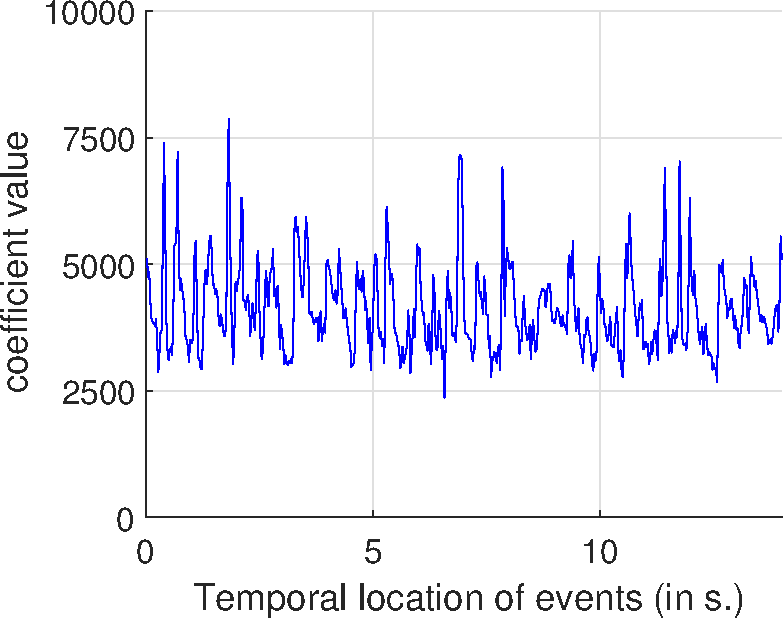
\includegraphics[width=.45\textwidth]{img/LLFs/Down_centroid}\label{fig:LLFs:down_centroid}} \hfil
	\subfloat[Spectral Centroid for \textit{Orinoco Flow}]{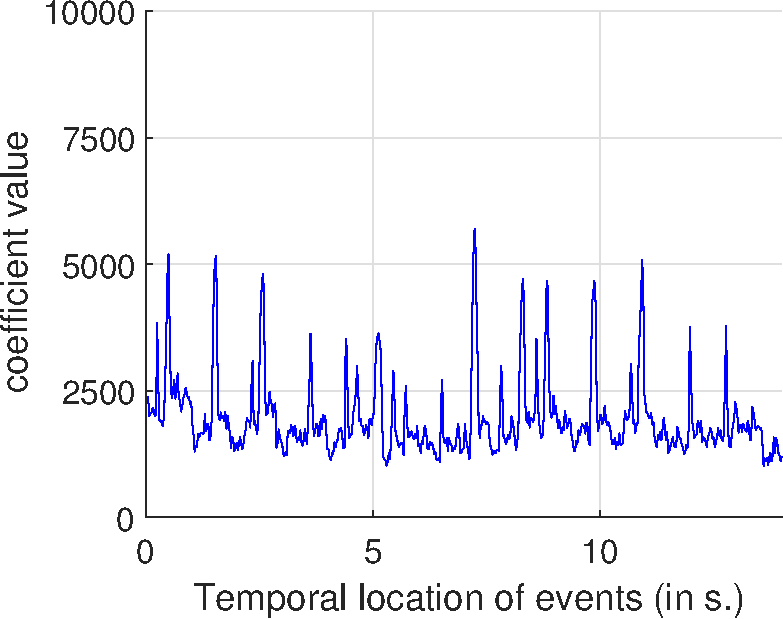
\includegraphics[width=.45\textwidth]{img/LLFs/Henya_centroid}\label{fig:LLFs:henya_centroid}}
	\caption{Spectral Centroid for the two songs. The red dashed line indicates the average of the values of the feature.}
	\label{fig:LLFs:centroid}          
\end{figure}

The \textit{Spectral Centroid} ($SC$) represents the ``center of gravity'' (first moment) of the magnitude spectrum, i.e., the frequency at which the energy of the spectrum is more concentrated \cite{weihs2016music}. The $SC$ is computed as:
\begin{equation}\label{eq:FSC}
SC_l = \frac{\sum\limits_{k=1}^{K}f(k)|S_l(k)|}{\sum\limits_{k=1}^{K}|S_l(k)|} \; ,
\end{equation}
where $K$ represents the total number of frequency bins, $f(k)=F_s \cdot k/L $ is the frequency corresponding to the $k$-th bin, $F_s$ is the sampling frequency of $s(n)$ and $L$ is the length of the frame in samples. The Spectral Centroid gives us an insight on where the frequency components of the magnitude spectrum are more distributed and hence which frequencies are likely to be perceived as predominant. The lower the Spectral Centroid, the darker the sound, and the higher the Spectral Centroid, the brighter the sound. For this reason, the Spectral Centroid can be seen as a descriptor of the brightness of the sound. The evolution of the Spectral Centroid over time for two reference songs are shown in figure \ref{fig:LLFs:centroid}. We notice that the average Spectral Centroid of \textit{Orinoco Flow} (Fig. \ref{fig:LLFs:henya_centroid}) is lower than in the \textit{Down with the Sickness} (Fig. \ref{fig:LLFs:down_centroid}), and therefore that \textit{Down with the Sickness} is brighter than \textit{Orinoco Flow}, which, when listening to the two songs, might seem counter-intuitive. However, it is worth remembering that we are considering a \textit{bright} or \textit{dark} sound from a timbral perspective, which should not be confused with the emotional perspective. In this case, the average Spectral Centroid in  \textit{Orinoco Flow} is around 2000 Hz, which can be due to various low-pitch harmonic instruments that play in the song. The high Centroid for \textit{Down with the Sickness}, instead, can be caused by high-pitch percussive sounds or electric guitars.

\begin{figure}[tb]
	\centering
	\subfloat[Spectral Spread for \textit{Down with the Sickness}]{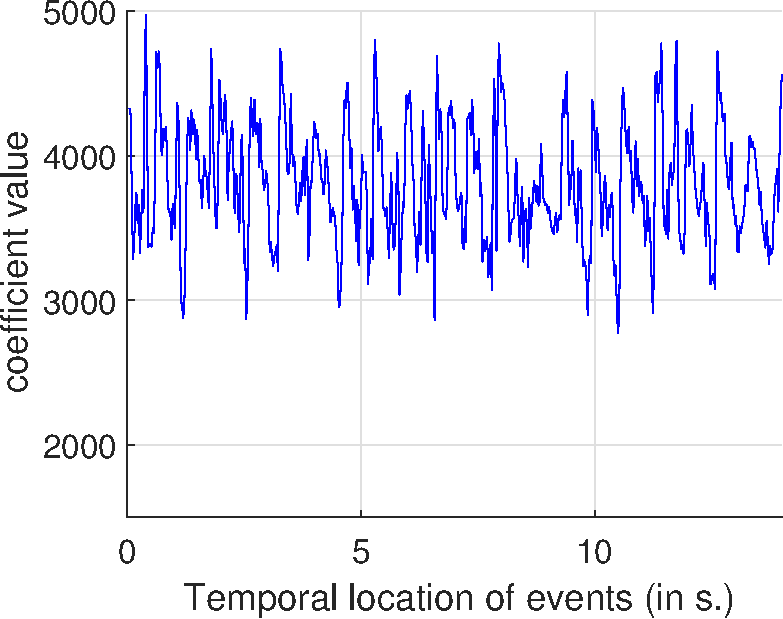
\includegraphics[width=.45\textwidth]{img/LLFs/Down_spread}\label{fig:LLFs:down_spread}} \hfil
	\subfloat[Spectral Spread for \textit{Orinoco Flow}]{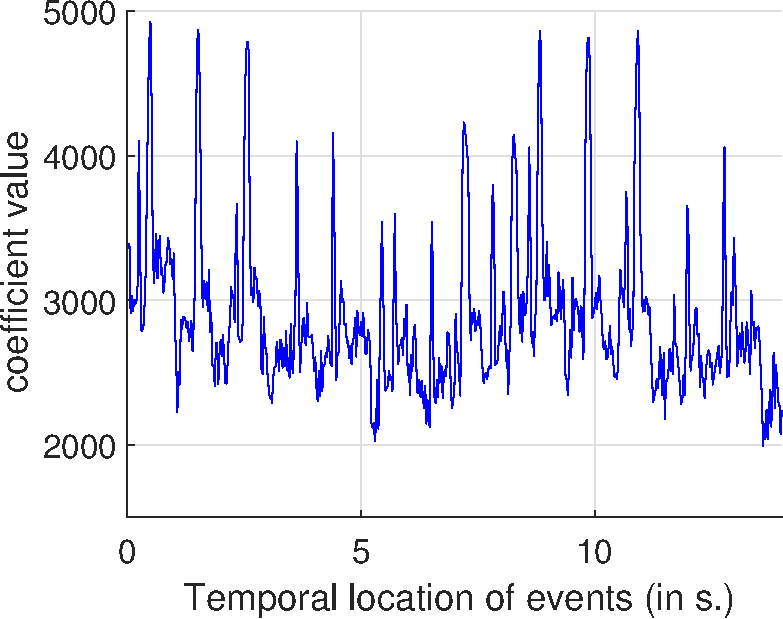
\includegraphics[width=.45\textwidth]{img/LLFs/Henya_spread}\label{fig:LLFs:henya_spread}}
	\caption{Spectral Spread for the two songs. The red dashed line indicates the average of the values of the feature.}
	\label{fig:LLFs:spread}          
\end{figure}

The second statisticalmoment of the distribution of the spectrum is the \textit{Spectral Spread} ($SSp$) and it measures the standard deviation of the spectrum from its frequency mean, i.e., from the Spectral Centroid. The Spectral Spread is computed as :
\begin{equation}\label{eq:FSS}
SSp_l = \sqrt{\frac{\sum\limits_{k=1}^{K}(f(k)-SC_l)^2 |S_l(k)|}{\sum\limits_{k=1}^{K}|S_l(k)|}} \;.
\end{equation}
The Spectral Spread captures how much the power of the spectrum is spread over the frequencies around the Spectral Centroid. The lower the $SSp$, the more the spectrum is distributed around its centroid and hence, the more it resembles a pure tone. On the contrary, a noisy sound is characterized by a more spread spectrum and therefore by high values of the Spectral Spread. While the noisiness and the Spectral Spread are not directly related, high values of the Spectral Spread might be used as an indicator of the noisiness of the audio signal. In Figure \ref{fig:LLFs:spread} we compare the Spread of the two songs. The average $Ssp$ values of \textit{Down with the Sickness} (Fig. \ref{fig:LLFs:down_spread}) are quite high, so we might assume that the distribution of the spectrum has a great variance, hence possibly sounding rather noisy. On the other side, from the lower values of \textit{Orinoco Flow} (Fig. \ref{fig:LLFs:henya_spread}), combined with the lower centroid seen in Figure \ref{fig:LLFs:henya_centroid}, we might assume that the song contains low-pitch and rather harmonic sounds.


\begin{figure}[tb]
	\centering
	\subfloat[Spectral Skewness for \textit{Down with the Sickness}]{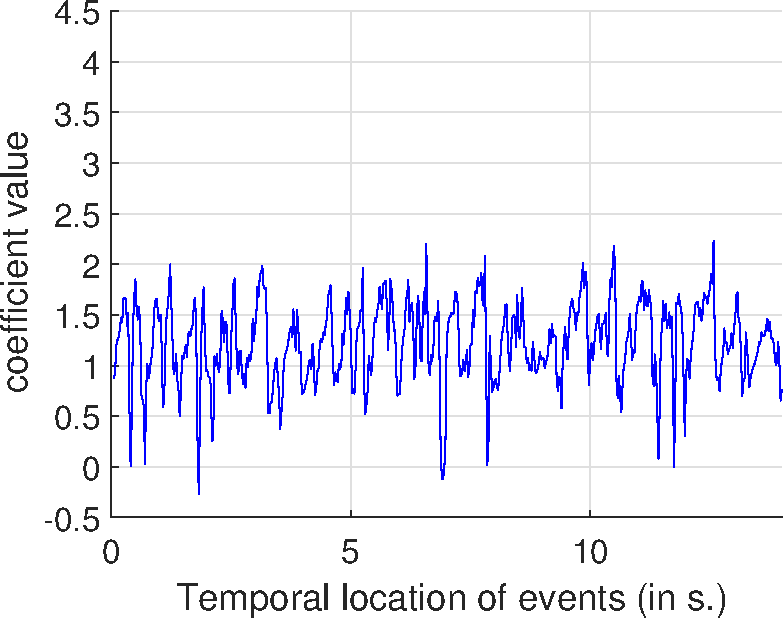
\includegraphics[width=.45\textwidth]{img/LLFs/Down_skewness}\label{fig:LLFs:down_skewness}} \hfil
	\subfloat[Spectral Skewness for \textit{Orinoco Flow}]{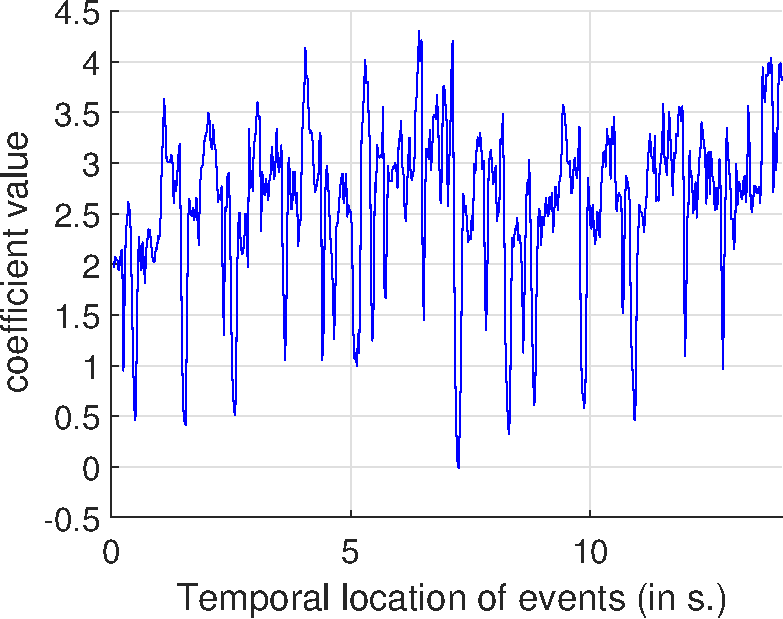
\includegraphics[width=.45\textwidth]{img/LLFs/Henya_skewness}\label{fig:LLFs:henya_skewness}}
	\caption{Spectral Skewness for the two songs. The red dashed line indicates the average of the values of the feature.}
	\label{fig:LLFs:skewness}          
\end{figure}

The third statistical moment is called \textit{Spectral Skewness} ($SSk$) and it computes the coefficients of the skewness of the frequency distribution, i.e., the degree of its symmetry around the Spectral Centroid \cite{Tanghe2005}:
\begin{equation}\label{eq:FSSK}
SSk_l = \frac{\sum\limits_{k=1}^{K}(f(k)-SC_l)^3\cdot |S_l(k)|}{K\cdot SSp_l^3} \; .
\end{equation}
An exactly symmetric frequency distribution results in a zero Spectral Skewness. Positive values of $SSk$ indicate a distribution of the spectrum energy with a longer or fatter tail toward the higher frequencies (with respect to the Spectral Centroid). Negative values of $SSk$ indicate a longer or fatter tail of the spectrum energy towards the lower frequencies. It is possible to include a normalization term in the term, in order to neglect the contribute of the energy of the signal \cite{weihs2016music}. However, we follow the approach of \cite{Tanghe2005}, since the Spectral Spread in the denominator represent the standard deviation of the distribution of the spectrum and it is already normalized with respect to its energy and to the length of the frame.

Together with the Centroid and the Spread, Spectral Skewness gives us an insight on the frequency distribution, but it is hard to derive a general interpretation from it. However, from the visualization in Figure \ref{fig:LLFs:skewness}, it is clear that the distribution of the Orinoco Flow's spectrum presents a tail toward the higher frequencies, (Fig. \ref{fig:LLFs:henya_skewness}), while \textit{Down with the Sickness} presents lower values and sometimes negative (Fig. \ref{fig:LLFs:down_skewness}), that indicates the distribution of the spectrum is more uniform than those from Oricono Flow.

\begin{figure}[tb]
	\centering
	\subfloat[Spectral Kurtosis for \textit{Down with the Sickness}]{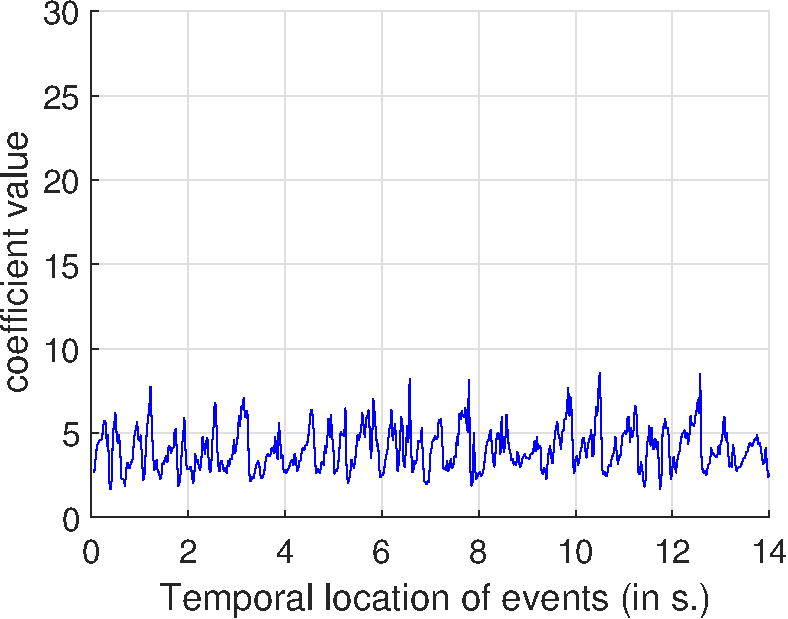
\includegraphics[width=.45\textwidth]{img/LLFs/Down_kurtosis}\label{fig:LLFs:down_kurtosis}} \hfil
	\subfloat[Spectral Kurtosis for \textit{Orinoco Flow}]{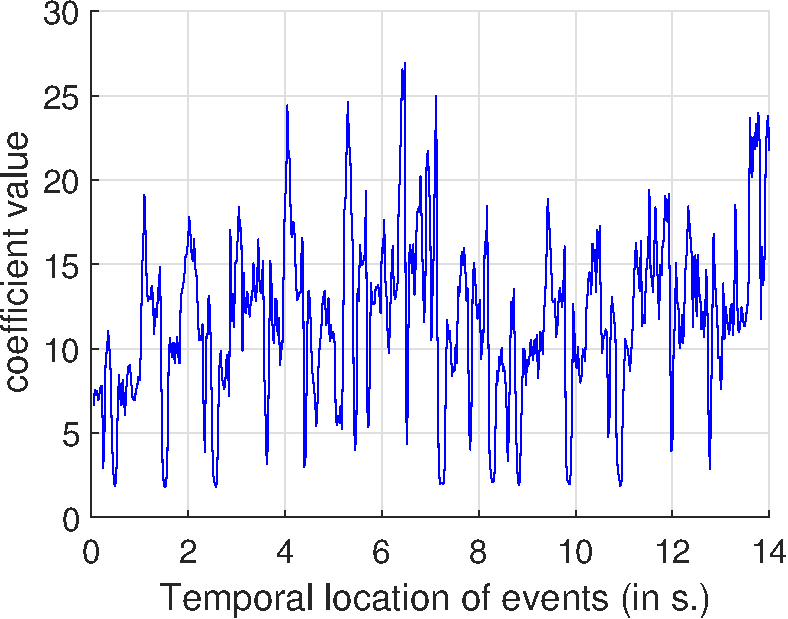
\includegraphics[width=.45\textwidth]{img/LLFs/Henya_kurtosis}\label{fig:LLFs:henya_kurtosis}}
	\caption{Spectral Kurtosis for the two songs. The red dashed line indicates the average of the values of the feature.}
	\label{fig:LLFs:kurtosis}          
\end{figure}

The fourth statistics moment is called \textit{Spectral Kurtosis} $SK$ and it indicates the resemblance of the spectral shape with a Gaussian bell curve \cite{weihs2016music}:
\begin{equation}\label{eq:FSK}
SK_l = \frac{\sum\limits_{k=1}^{K} (f(k)-SC_l)^4 |S_l(k)| }{K \cdot SSp_l^4} -3 \; .
\end{equation}
A frequency distribution with a perfect bell-curved shape results in zero Spectral Kurtosis, thanks to the $-3$ offset. Positive values of $SK$ indicates that the spectral shape presents a strong peak around the Spectral Centroid, while sub-Gaussian shapes, tending toward a uniform distribution, exhibit negative values. The Spectral Kurtosis can be interpreted as an indication of the bandwidth of the spectrum, from wide-band sounds (negative values) to narrow-band sounds (positive values). It is clear from Figure \ref{fig:LLFs:kurtosis} that the distribution of the spectrum of \textit{Orinoco Flow} presents a peaked spectral shape around the centroid(Fig. \ref{fig:LLFs:henya_kurtosis}), while \textit{Down with the Sickness} closely resembles a uniform distribution, and therefore presents a band wider than the \textit{Orinoco Flow}'s one.(Fig. \ref{fig:LLFs:down_kurtosis}).


Two more spectral features are the \textit{Spectral Entropy} ($SE$) \cite{Lartillot2007}, and \textit{Spectral Flatness} ($SF$) \cite{Kim2005}, both providing an indicator of the noisiness of the sound.

\begin{figure}[tb]
	\centering
	\subfloat[Spectral Entropy for \textit{Down with the Sickness}]{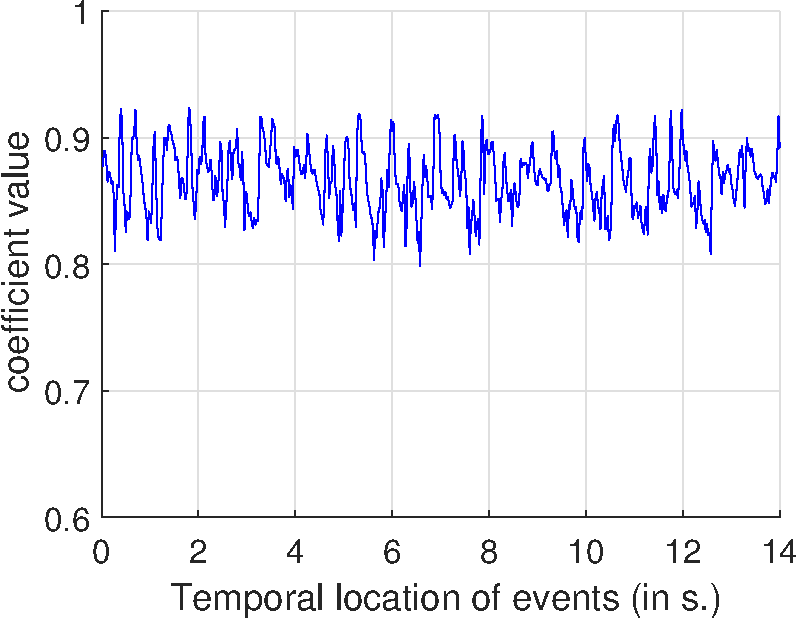
\includegraphics[width=.45\textwidth]{img/LLFs/Down_entropy}\label{fig:LLFs:down_entropy}} \hfil
	\subfloat[Spectral Entropy for \textit{Orinoco Flow}]{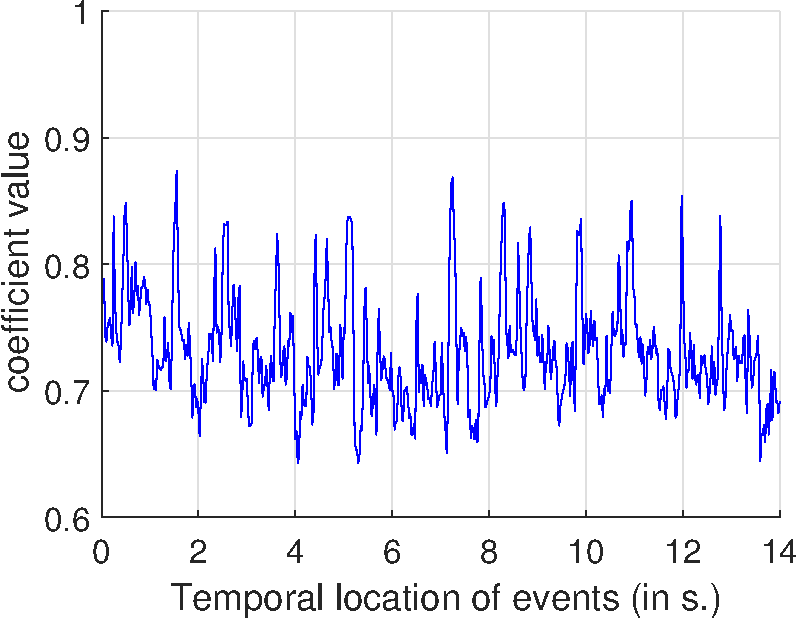
\includegraphics[width=.45\textwidth]{img/LLFs/Henya_entropy}\label{fig:LLFs:henya_entropy}}
	\caption{Spectral Entropy for the two songs. The red dashed line indicates the average of the values of the feature.}
	\label{fig:LLFs:entropy}          
\end{figure}

The \textit{Spectral Entropy} ($SE$) applies the Shannon's entropy definition \cite{shannon2001}, commonly used in information theory context to estimate the amount of information encoded in a distribution of symbols. The Spectral Entropy is commonly computed \cite{Lartillot2007} with a factor of normalization that provides an estimation which is independent on the length of the frame:
\begin{equation}
SE_l = -\frac{\sum\limits_{k=1}^{K}|S_l(k)|\log |S_l(k)|}{\log K}.
\end{equation}
The spectral entropy captures the uncertainty of the distribution of the energy values of the spectrum and hence its flatness. The maximum entropy is indeed obtained with a perfect flat spectrum, while the minimum entropy is given by a very sharp peak in the spectrum with a low background noise. This is the reason why the Spectral Entropy is used as an indicator of the noisiness of the sound.

\begin{figure}[tb]
	\centering
	\subfloat[Spectral Flatness for \textit{Down with the Sickness}]{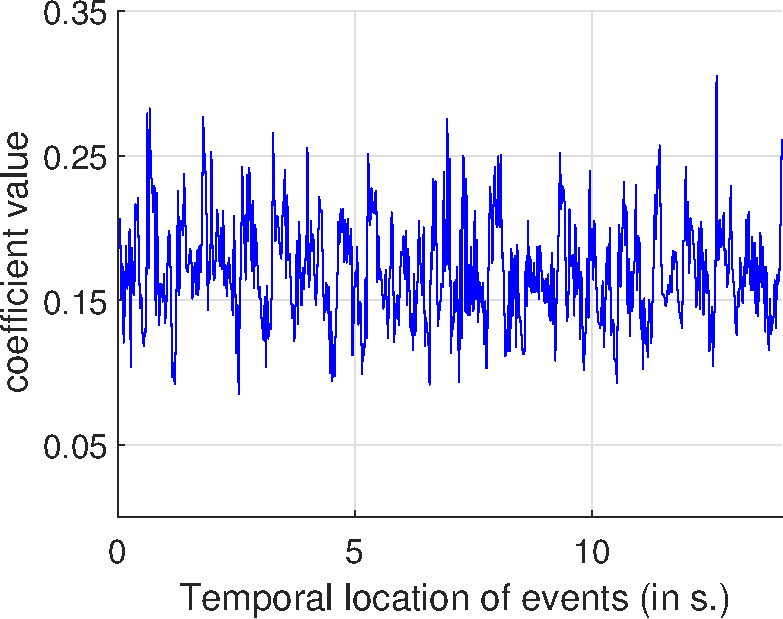
\includegraphics[width=.45\textwidth]{img/LLFs/Down_flatness}\label{fig:LLFs:down_flatness}} \hfil
	\subfloat[Spectral Flatness for \textit{Orinoco Flow}]{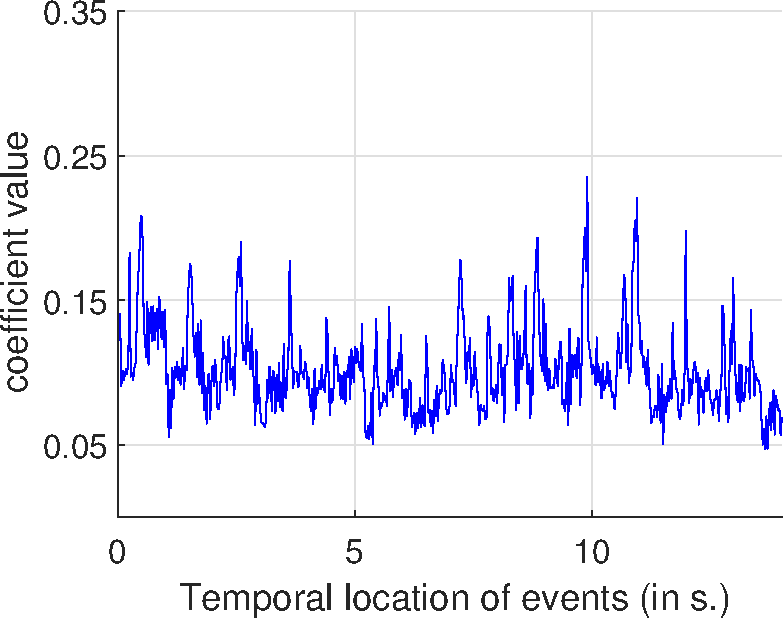
\includegraphics[width=.45\textwidth]{img/LLFs/Henya_flatness}\label{fig:LLFs:henya_flatness}}
	\caption{Spectral Flatness for the two songs. The red dashed line indicates the average of the values of the feature.}
	\label{fig:LLFs:flatness}          
\end{figure}

The \textit{Spectral Flatness} ($SF$) is an indicator of the degree of flatness of the spectrum and is therefore used as an estimate of the noisiness of the sound \cite{Rottondi2015}. It is computed as the ratio between the geometric and the arithmetic mean
\begin{equation}
SF_l = K \frac{\sqrt[K]{\prod\limits_{k=1}^{K}|S_l(k)|}}{\sum\limits_{k=1}^{K}|S_l(k)|},
\end{equation}
which provides an estimation of the similarity between the magnitude spectrum of the signal frame and the flat shape inside a predefined frequency band. 


A visualization of Spectral Entropy and Spectral Flatness is shown in Figures \ref{fig:LLFs:entropy} and \ref{fig:LLFs:flatness} respectively. Both features capture higher values of noisiness for \textit{Down with the Sickness} than for Orinoco Flow, which is confirmed by the listening of the two pieces.
 Given a generic amplitude of a frame of a STFT $|S_l|$, the MFCCs are computed by performing the following processing. In the following, we will neglect the notation of the $l$-th frame for the sake of clarity. First, a mel-filter bank, i.e., a filter bank whose bands model the auditory response of the cochlea, is applied to the frame. The mel scale follows the logarithmic perception of the frequencies, so there are more filter banks in the lower frequencies than in the higher ones. The log-\textit{Power Spectrum} $E_k$ is computed for each of the band of the mel-filter bank, where the logarithmic scale is used in order to take the human perception of loudness into consideration. Finally, the Discrete Cosine Transform (DCT) is applied to the Power Spectrum in order to extract a complete yet compact representation of it:
\begin{equation}
%\begin{array}{rcl} 
c_i = \sum_{k=1}^{N_c}  \log(E_k) \cos \left[i \left(k-\frac{1}{2}\right) \frac{\pi}{N_c} \right]  \;\text{ with }\; 1\leq i\leq K_c, 
%\end{array}
\end{equation}
where $c_i$ is the $i-th$ MFCC component, $E_k$ is the spectral energy measured in the critical band of the $i-th$ mel-filter, $N_c$ is the number of mel-filters and $K_c$ is the amount of cepstral coefficients extracted from each frame, which is typically 13. Back to the indication of the frames, the vector $\mathbf{c_l}$, is composed of the $K_c$ cepstral coefficients computed for the $l-th$ frame, as a compact descriptor of the timbre of the underlying sound. The MFCCs extracted from the two songs of examples are shown in Figure \ref{fig:LLFs:mfcc}. 


%The pooling of the frames can also be used to embed other information from the signal, such as the musicological aspects. In the foll Another pooling approach concerns to use the information from music rhythm to create a feature representation that also embeds some musical aspects. In order to do so, we need to extract some features from the signal domain that provide a representation of such musical aspects, by means of the Mid-Level Features described in the following Section.

\begin{figure}[tb]
	\centering
	\subfloat[MFCCs for \textit{Down with the Sickness}]{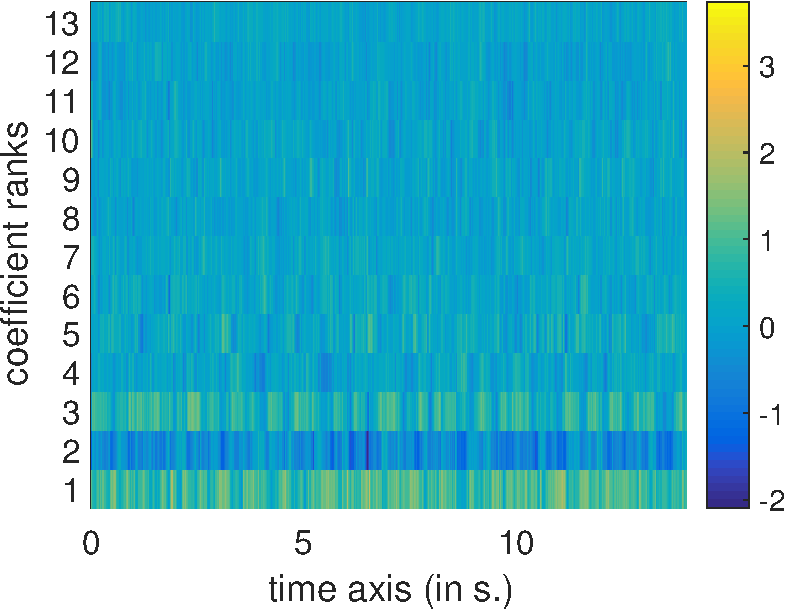
\includegraphics[width=.45\textwidth]{img/LLFs/Down_mfcc}\label{fig:LLFs:down_mfcc}} \hfil
	\subfloat[MFCCs for \textit{Orinoco Flow}]{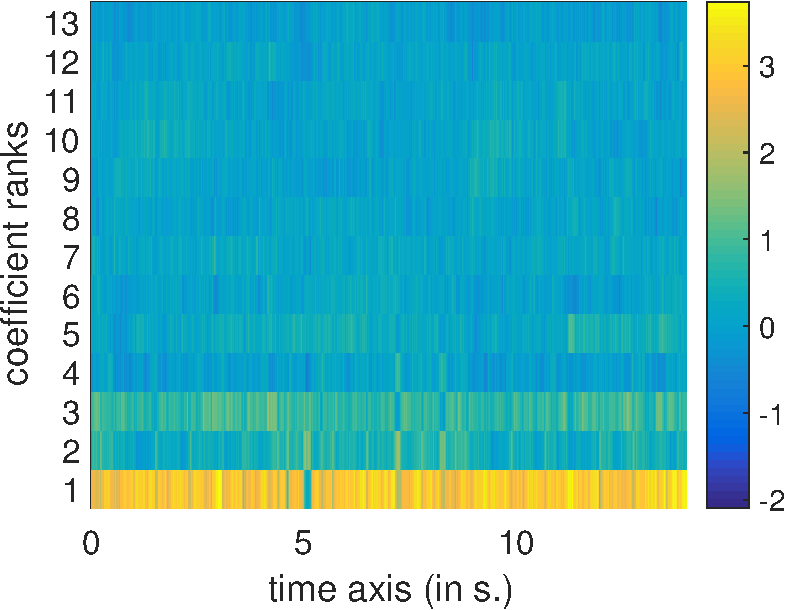
\includegraphics[width=.45\textwidth]{img/LLFs/Henya_mfcc}\label{fig:LLFs:henya_mfcc}}
	\caption{MFCCs for the two songs.}
	\label{fig:LLFs:mfcc}          
\end{figure}


\begin{figure}[tb]
	\centering
	\subfloat[Chromagram for \textit{Down with the Sickness}]{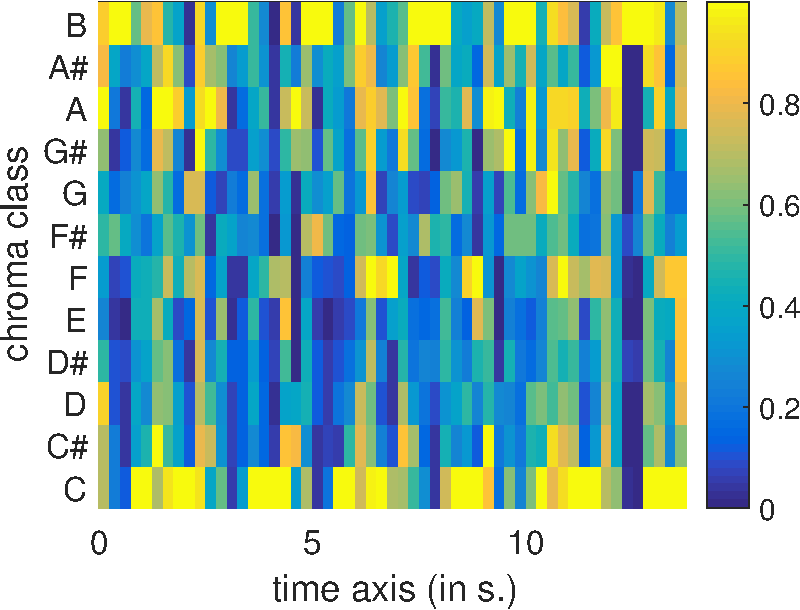
\includegraphics[width=.45\textwidth]{img/LLFs/Down_chroma}\label{fig:LLFs:down_chroma}} \hfil
	\subfloat[Chromagram for \textit{Orinoco Flow}]{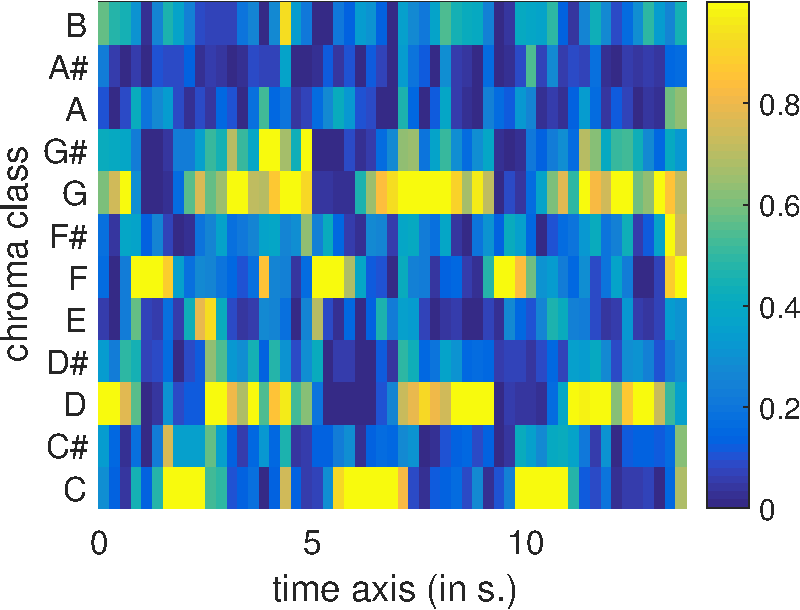
\includegraphics[width=.45\textwidth]{img/LLFs/Henya_chroma}\label{fig:LLFs:henya_chroma}}
	\caption{Chromagram for the two songs.}
	\label{fig:LLFs:chroma}          
\end{figure}


With regard to the MLFs, the most widely used tonal descriptors are the \textit{chroma} features, also called \textit{Pitch Class Profile} (PCP), which represent the distribution of pitch classes in a certain frame of analysis, and the \textit{chromagram}, which collect the chroma features through the frames of a song. In the equal tempered scale, which is the main scale used in Western popular music, two notes belong to the same pitch class when the ratio of their fundamental frequencies is an integer power of two (e.g., $f_1=f$, $f_2=2f$). The equal tempered scale consists of twelve pitch classes, each of which is identified with a name, from C to B through the semi-tones. When shifting a melody by an octave (i.e., doubling or halving the frequency of the notes), in fact, the melody keeps the same harmony and key of the original. It is reasonable therefore to summarize the harmonic content of a song by considering the pitch classes of the notes, regardless of the original octave.


The chroma features are built by first applying a filter bank to the log-magnitude spectrum of a frame, with the filters' bands centered in the fundamental frequencies of the notes from the equal tempered scale. The results of the pass-band filters are then collapsed in a 12-bin histogram-like structure where each bin represents a pitch class. The chroma features and the collected chromagram are often the first step for further processing regarding chord or harmony recognition or music structure analysis \cite{Nieto2D, Digiorgi2013}. A visual representation is shown in Figure \ref{fig:LLFs:chroma}. The presence of harmonic sounds in \textit{Orinoco Flow} allows us to clearly see the predominant notes in the chromagram (Fig \ref{fig:LLFs:henya_chroma}), while the chromagram extracted from \textit{Down with the Sickness} appears more confused (Fig \ref{fig:LLFs:down_chroma}).

\begin{figure}[tb]
	\centering
	\subfloat[Tempo for \textit{Down with the Sickness}]{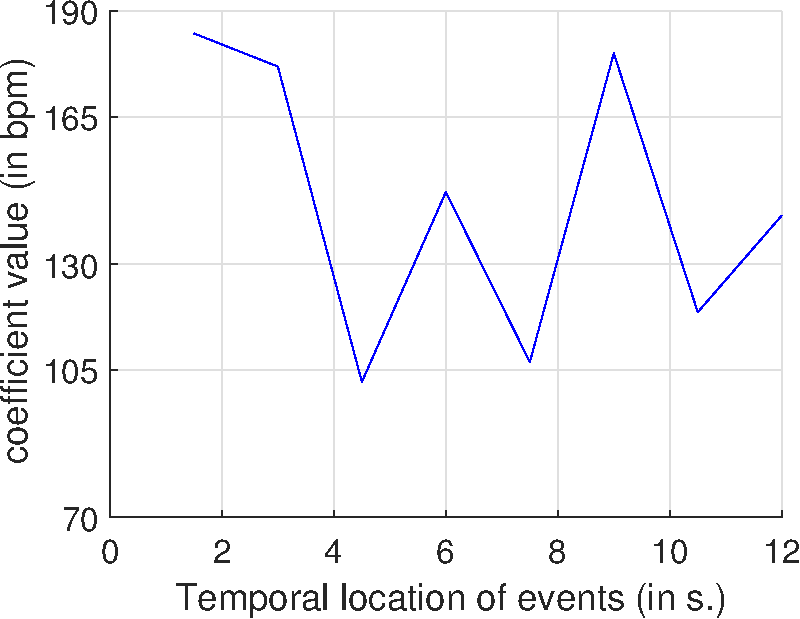
\includegraphics[width=.45\textwidth]{img/LLFs/Down_tempo}\label{fig:LLFs:down_tempo}} \hfil
	\subfloat[Tempo for \textit{Orinoco Flow}]{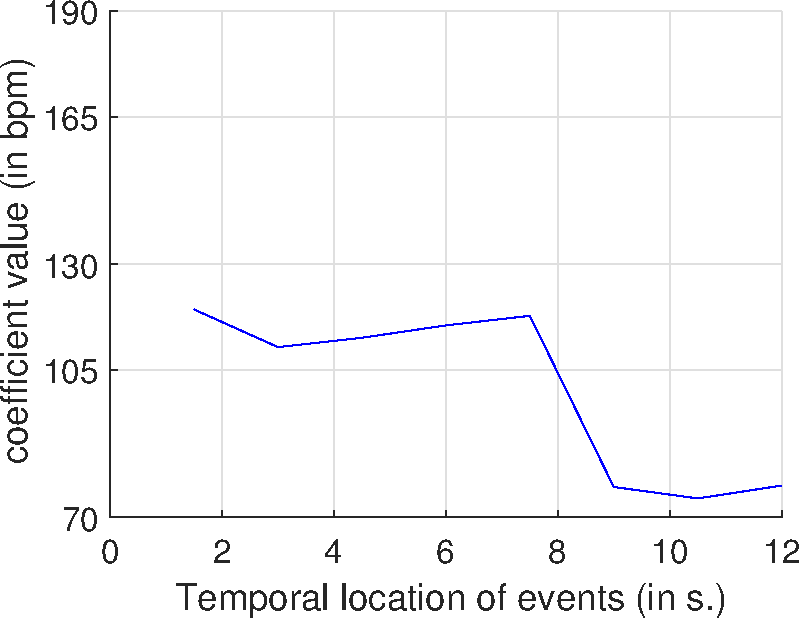
\includegraphics[width=.45\textwidth]{img/LLFs/Henya_tempo}\label{fig:LLFs:henya_tempo}}
	\caption{Tempo for the two songs. The red dashed line indicates the average of the values of the feature.}
	\label{fig:LLFs:tempo}          
\end{figure}

With respect to rhythmic features, one of the most widely used feature is the \textit{tempo}, which represents the speed of execution of a given piece. As a descriptor, tempo is correlated with other semantic features \cite{Buccoli2013}, e.g., related to mood or dynamics: a piece with a slow tempo is more likely to be described as \textit{calm}, or \textit{romantic}, while a faster tempo can be correlated with more active moods. Tempo is specified in beats per minute (BPM), i.e., how many beats must be played in a minute, where the beats are defined as  \textit{the temporal unit of a composition, as indicated by the (real or imaginary) up and down movements of a conductor's hand}\cite{harvardDictionary}. We can estimate the instantaneous tempo computing the time interval between two consecutive beats, or we can estimate the tempo over longer time windows. For example, in the Figure \ref{fig:LLFs:tempo} we show an analysis of tempo over 3 second-windows with 50\% overlap, from which we can infer that \textit{Orinoco Flow} is slower than \textit{Down with the Sickness} (Figures \ref{fig:LLFs:down_tempo}, \ref{fig:LLFs:henya_tempo}). Figure \ref{fig:LLFs:tempo} also highlights the difficulty of the task of automatic mid-level feature modeling and extraction, since the estimated tempo is quite unstable, while the real tempo of the excerpts is not. 

In this thesis we also uses two rhythmic features as indicators of the rhythmic complexity of a music piece: the \textit{Event Density} and the \textit{Rhythmic Complexity}. Both indicators analyze the rhythm by considering only the the \textit{onsets} of the notes and their occurrence in the context of the general music score. For this reason, these metrics are computed from a symbolic representation of the score, rather than from the audio signal. 

The \textit{Event Density} ($ED$) is defined in \cite{Lartillot2007} as the average number of onsets per second:
\begin{equation}
ED = \frac{NO}{T},
\label{eq:LLFs:ED}
\end{equation}
where $NO$ is the number of onsets and $T$ is the duration of the musical piece. In order to 
make the $ED$ values for polyphonic parts comparable with the ones computed over monophonic parts or with purely percussive parts, when several notes are played in the same instant, e.g., in a chord, they are counted as one onset.  

The \textit{Rhytmic Complexity} ($RC$) \cite{povel} estimates the complexity of the rhythmic pattern of a part as a weighted sum of different factors that are believed to contribute to make a part rhytmically complex. The Rhytmic Complexity is computed as: 
\begin{equation}\label{eq:RC}
RC= w_1 \; H + w_2 \; ED + w_3 \; \sigma + w_4 \; A,
\end{equation}
where $w_1, \ldots, w_4$ are the tunable weights of the sum. 
The computation of $RC$ involves, as a first step, to compute the distribution of the duration of the notes. In Equation \ref{eq:RC}, $H$ is the entropy and $\sigma$ is the standard deviation of such a distribution \cite{eerola2003}, $ED$ is the Event Density as defined in Equation \ref{eq:LLFs:ED}. $A$ measures the synchrony of phenomenal accents in the part and in the metrical hierarchy. The metrical hierarchy of phenomenal accents refers to the natural decomposition of a rhythmic pattern into strong and weak accents performed by a musician and induced by the sheet music, e.g., the strong accents in the first beat of the bars. Trained musicians are used to this metrical hierarchy and it is easy for them to follow it. The phenomenal accents in the part refer to where the composer chose to place the accents in the part in order to induce a certain emotion or to express a specific expression. The misalignment between the two systems of accents, which is captured by $A$, adds some complexity in the execution for the musicians. 

In the MIDI toolbox \cite{Eerola2004}, the weights are defined as $w_1= 0.7$, $w_2=0.2,$  $w_3=0.5$, $w_4=0.5$, i.e., the Entropy of the distribution of the notes has the greatest relevance, then the standard deviation of the distribution of the notes and the synchrony of phenomenal accent in the score are equally weighted and finally, the Event Density receives a low weight. 
%
\section{Learned Features}\label{sec:app:learned}
In this Section, we provide the technical background of the unsupervised deep learning architecture we use in this work, the \textit{Deep Belief Network}, which is composed by stacking several layers of a 2-layer neural networks called \textit{Restricted Boltzmann Machine}. 

\subsection{Restricted Boltzmann Machines}\label{sec:Bootleg:deep}
A Restricted Boltzmann Machine (RBM) is an \textit{energy-based} generative model, i.e., a model that associates a scalar energy to each configuration of the variables of interest, by assigning lower values to the samples that are likely to belong to that distribution. More formally, the energy-based models define a probability distribution through an energy function:
\begin{equation}
P(x)=\frac{e^{-\E(x)}}{Z},
\label{eq:probEnergy}
\end{equation}
where $Z$ is a normalization factor called \textit{partition function}, defined as 
\begin{equation}
Z=\sum_{\tilde{x}} e^{-\E(\tilde{x})},
\end{equation}
whose sum (or integral, if $x$ is continuous) spans the input space. The training of an energy-based model corresponds to shape the energy function such that low energy values are associated to plausible configurations, i.e., configurations of the input variable that are more likely to occur.

The energy function have different formulations. A common formulation computes the energy function as a sum of components, where each component is called \textit{expert} $f_i$:
\begin{equation}
\E(x)=\sum_i f_i(x)
\end{equation}
\begin{equation}
\text{so that }P(x)\propto=\prod_i P_i(x) \propto \prod_i e^{-f_i(x)}.
\label{eq:HLFs:experts}
\end{equation}
The probability distribution is therefore modeled as a \textit{product of experts}, where each expert $P_i(x)=e^{-f_i(x)}$ can be seen a detector of implausible configurations of $x$: if $x$ is implausible and then some $P_i(x)=0$, the total $P(x)=0$. With this formulation, each expert behaves as a constraint, which makes the Energy model a distributed representation.

\begin{figure}[tbp]
	\centering
	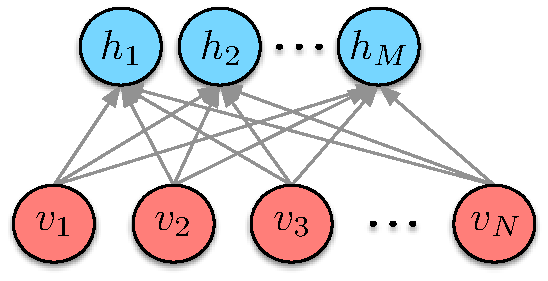
\includegraphics[width=0.6\columnwidth]{img/Bootleg/RBM_scheme_latexit.pdf}
	\caption{Restricted Boltzmann Machine topology.}
	\label{fig:Bootleg:RBMScheme}
	\vspace{-1em}
\end{figure}

The RBM is structured as a two-layer network of neurons: i) a visible layer $\mathbf{v} \in \mathbb{R}^{N}$ (the input layer); ii) a hidden layer $\mathbf{h} \in \mathbb{R}^{M}$, where $N$ and $M$ are the number of visible and hidden neurons respectively, which is decided in the architecture design step. Neurons in different layers are fully connected, whereas no connection exists between neurons of the same layer. The probability distribution is hence formalized as 
\begin{equation}
P(\mathbf{v},\mathbf{h})=\frac{e^{-\E(\mathbf{v},\mathbf{h})}}{Z},
\end{equation}
but, since only $\mathbf{v}$ is observed, we care about the marginal probability:
\begin{equation}
P(\mathbf{v})=\sum_\mathbf{h} \frac{e^{-\E(\mathbf{v},\mathbf{h})}}{Z},
\end{equation}
with a sum over all the hidden space (i.e., the hidden variables $\mathbf{h}$ that can occur jointly with $\mathbf{v}$).

We introduce the notation of \textit{free energy} to have a notation similar to the one of Eq. \ref{eq:probEnergy}:
\begin{equation}
P(\mathbf{v})=\frac{e^{-\FE(\mathbf{v})}}{\sum_{\tilde{\mathbf{v}}}e^{-\FE(\tilde{\mathbf{v}})}},
\end{equation}
\begin{equation}
\text{with }\FE(\mathbf{v})=-\log\sum_\mathbf{h} e^{-\text{Energy}(\mathbf{v},\mathbf{h})}
\label{eq:LLFs:freeenergy}
\end{equation}

In an RBM, the energy function for a configuration of input and hidden variable, is defined as \cite{Bengio2009}
\begin{equation}
\E(\mathbf{v},\mathbf{h}) = -\mathbf{b}^\top\mathbf{v} -\mathbf{c}^\top\mathbf{h}-\mathbf{h}^\top\mathbf{W}\mathbf{v},
\label{eq:HLFs:energyRBM}
\end{equation}
where $^\top$ indicates the transpose of a vector, while $\mathbf{b} \in \mathbb{R}^{N \times 1}$, $\mathbf{c} \in \mathbb{R}^{M\times 1}$, and $\mathbf{W} \in \mathbb{R}^{M \times N}$ are the parameters of the network. %To find the aforementioned parameters (i.e., $\mathbf{W}$, $\mathbf{b}$, and $\mathbf{c}$), 
In the RBM, the free energy function is defined as \cite{Bengio2009}
\begin{equation}
\FE(\mathbf{v}) = -\log \sum_{\mathbf{h} \in \mathcal{H}_\mathbf{v}}e^{-\E(\mathbf{v},\mathbf{h})},
\end{equation}
where the sum is extended to the set $\mathcal{H}_\mathbf{v}$ of possible outputs $\mathbf{h}$, given an input $\mathbf{v}$ (i.e., we make some hypotheses on possible vectors $\mathbf{h}$ associated to a vector $\mathbf{v}$). 

The Free Energy then becomes: 
\begin{equation}
\FE(\mathbf{v})=-\mathbf{b}\T \mathbf{v} -\sum_i \log \sum_{h_i} e^{\mathbf{h}_i \mathbf{W}_i \mathbf{v}}
\end{equation}
and the conditional probability $P(\mathbf{h}|\mathbf{v})$ is now very easily tractable:
\begin{equation}
P(\mathbf{h}|\mathbf{v})=\prod_i P(\mathbf{h}_i|\mathbf{v}).
\end{equation}
The conditional distribution can be seen as a product of experts as in Eq. \ref{eq:HLFs:experts}, where each hidden neuron is an expert that partitions the input space. The conditional probability of the hidden variable $\mathbf{h}$ is simply a product of the conditional probabilities of the single units, i.e., we obtain the output for each of the hidden unit as  
\begin{equation}
P(\mathbf{h}_i|\mathbf{v})= \text{sigm}(\mathbf{c}_i + \mathbf{W}_i \mathbf{v}),
\end{equation}
where the $\text{sigm}(\mathbf{x})=(1+exp(-\mathbf{x}))^-1$ is the sigmoid function applied element-wise. Since the energy is symmetric (from Eq.\ref{eq:HLFs:energyRBM}), we can easily state that 
\begin{equation}
P(\mathbf{v}|\mathbf{h})=\prod_i P(\mathbf{v}_i|\mathbf{h})
\label{eq:LLFs:generatingx}
\end{equation} and $P(\mathbf{v}_i|\mathbf{h})= \text{sigm}(\mathbf{b}_i + \mathbf{W}\T_{.j} \mathbf{v})$, where $\mathbf{W}_{.j}$ is the $j$-th column of $\mathbf{W}$. 

%More formally, let us consider the vector $\mathbf{v} \in \mathbb{R}^{N\times 1}$ representing the data under analysis (e.g., samples of the spectrum of an audio excerpt), and the vector $\mathbf{h} \in \mathbb{R}^{M\times 1}$ representing the output of the RBM whose input is $\mathbf{v}$. Each neuron of the visible layer is a sample of $\mathbf{v}$, while each neuron of the hidden layer is a sample of $\mathbf{h}$. The goal of training an RBM is to find the parameters of the network that enable to compute $\mathbf{h}$ (i.e., our feature vector) from $\mathbf{v}$ (i.e., our data), so that $\mathbf{h}$ contains salient information that characterizes $\mathbf{v}$.
%With this in mind, and 
Given a set $\mathcal{V}$ of training data vectors $\mathbf{v}$, the network parameters are estimated as 
\begin{equation}
\{\hat{\mathbf{W}}, \hat{\mathbf{b}}, \hat{\mathbf{c}}\} = \argmin{\mathbf{W}, \mathbf{b}, \mathbf{c}} \prod_{\mathbf{v} \in \mathcal{V}} F(\mathbf{v}).
\label{eq:training}
\end{equation}
In other words, we search for the parameters of the network that better explain all the possible hypothesized outputs.

In order to find the network parameters to shape the Energy Function, different iterative algorithms can be applied. The most widely used, thanks to its relatively low computational cost is the Contrastive Divergence ($CD-k$) algorithm. A proper iterative algorithm would need a full Monte-Carlo sampling of the hidden space, which is not tractable. The $CD-k$ algorithm offers an easier solution by using an approximation in the computation of the Free Energy and exploiting the generative power of the RBM. 

The Free Energy is supposed to be estimated over all the possible hidden configuration given a certain input, as defined in \ref{eq:LLFs:freeenergy}. Instead, the sum over the space of the hidden configurations is substituted with a single sample, the one given by the parameters at the $j$-th iterative step  $\{\hat{\mathbf{W}}^{(j)}, \hat{\mathbf{b}}^{(j)}, \hat{\mathbf{c}}^{(j)} \}$. This will introduce variance in the approximation of the gradient, which is however reduced by constantly updating the parameters with the iterative procedure.

With regards to the generative power of the RBM, from a configuration of the hidden variable $h$ we generate a new sample $x$ as defined in Equation \ref{eq:LLFs:generatingx}. A Gibbs Sampling is then performed by starting with a real visible input $v=x^{(0)}$, from which we generate $h^{(0)}$, that generates $x^{(1)}$, and so on:
%\begin{equation}
%\begin{array}{c}
\begin{align*}
x^{(0)} \sim \hat{P}(x)\\
h^{(0)} \sim P(h|x^{(0)})\\
x^{(1)} \sim P(x|h^{(0)})\\
...\\
x^{(k)} \sim P(x|h^{(k-1)}),
\end{align*}
%\end{array}
%\end{equation}
where  $\hat{P}$ is the empirical distribution, i.e., the distribution of the input, whereas $P$ is the model distribution.
The $CD-k$ algorithm performs $k$ sampling steps to generate a new sample. Since this sample has been generated by the model, it is less likely to belong to the empirical distribution. We want to shape the energy function in order to have low values for variables from the input data, which belong to the empirical distribution. The $CD-k$ algorithm considers the generated data $x^{k>0}$ as negative samples, and it shapes the energy function to obtain higher values where generated samples are more highly distributed. While higher $k$ achieves better performance, $CD-k$ has proven to be effective even with $k=1$ \cite{Bengio2009}.

The vector of hidden neurons $\mathbf{h}$ are used as a representation of the input vector $\mathbf{v}$ containing the most salient information about it. However, RBM has only one representation layer, that cannot extract abstract information from the signal. The Deep Belief Network provides such depth of representation.

% ----- DBN -----
\subsection{Deep Belief Network}
A Deep Belief Network (DBN) \cite{Hinton2006} is a deep learning network architecture that is built as the stack of Restricted Boltzmann Machines (RBMs) on top of each other. Each layer $k$ takes as input the hidden vector $\mathbf{h}^{(k-1)}$ of the previous one (as in Fig.~\ref{fig:LLFs:DBN}) in order to produce the more abstract features $\mathbf{h}^{(k)}$. The optimal number of layers (i.e., its \textit{depth} $K$) and the number of nodes for each layer $H^{(k)}$ depends on the problem that the network is designed to address, and it is difficult to be defined a-priori. The more the neurons and the deeper the network, the better the performance but also the more expensive the training of the network.


A DBN is trained by individually training the RBMs of which it is composed. First, the bottom layer is trained with the samples of the training set $\mathcal{V}$, obtaining the representation set
$$\mathcal{H}^{(1)}=\{P(\mathbf{h}|\mathbf{v}) \; \forall \mathbf{v} \in \mathcal{V}\}.$$ 
Then, $\mathcal{H}^{(1)}$ is fed to the RBM in the second layer in order to train it, generating the representation set $\mathcal{H}^{(2)}$, and so on for all the layers. 

This kind of architecture allows the RBMs in the top layers to combine the properties learned in the lower layers in order to provide a more abstract representation of the input data. Given a new data input $\mathbf{v}$, the output of the DBN is its multi-layer representation, i.e., the collection of all the hidden layers  $\mathbf{h}^{(k)}$ with $k=1,...K$, each one providing a different level of abstraction.

\section{Latent Semantic Analysis}\label{app:LSA}
%\subsection{Latent Semantic Analysis}
The Latent Semantic Analysis (LSA) is a technique that makes use of the Singular Value Decomposition to find an approximation of a annotated dataset. Let us define a dataset $\mathcal{D}=\{\mathbf{d}_1,...,\mathbf{d}_N\}$ of $N$ items, where each item is defined as a vector of $M$ terms belonging to the vocabulary $\mathcal{V}=\{v_1, ..., v_M\}$:
\begin{equation}
\mathbf{d}_i=[ w_{i,1}, ..., w_{i,M} ]\T \forall i=1,...,N, 
\end{equation}
where $w_{i,j}$ represents the weight of the descriptor $v_j$ for the item $\mathbf{d}_i$. In the categorical approach, $w_{i,j}\in\{0,1\}$, i.e., it is $1$ if the $j$-th HLF is used in the description of the $i$-th item and $0$ otherwise. In the social tagging scenario, a dimensional weight can be inferred by counting how many users used the $j$-th tag to describe the $i$-th item, or by using other approaches, leading to $w_{i,j}\in[0,1]$. 

We can now collect all the annotated items into the matrix $\mathbf{A}=[w_{i,j}]=[\mathbf{d}_1,...,\mathbf{d}_N] \in \mathbb{R}^{M\times N}$. 
The matrix $\mathbf{A}$ is usually sparse, since a full annotation requires a huge amount of annotations which are expensive to be collected and demand too high of a cognitive load. The LSA involves to compute the Singular Value Decomposition (SVD) of \textbf{A} \cite{dumais2004latent}:
\begin{equation}
\mathbf{A}=\mathbf{U} \mathbf{\Sigma} \mathbf{V}\T,
\end{equation}
where 
\begin{itemize}
	\item $\mathbf{\Sigma}\in \mathbb{R}^{M\times N}$ is the diagonal matrix of singular values, i.e., the eigenvalues of $\mathbf{A}\mathbf{A}\T$ and of $\mathbf{A}\T \mathbf{A}$ ;
	\item $\mathbf{U}\in \mathbb{R}^{M\times M}$ is the matrix collecting, as columns, the left-singular vectors of $\mathbf{A}$, i.e., the eigenvectors of  $\mathbf{A} \mathbf{A}\T$;
	\item $\mathbf{V}\in \mathbb{R}^{N\times N}$ is the matrix collecting, as columns, the right-singular vectors of $\mathbf{A}$, i.e., the eigenvectors of $\mathbf{A}\T \mathbf{A}$.
\end{itemize}

The columns of $\mathbf{U}$ represent a rotation of the axis from the descriptors in the vocabulary $\mathcal{V}$ to a linear combination of the descriptors in the most informative directions \cite{PAMI}. Such columns are orthogonal, so each direction is independent. The new space spanned by $\mathbf{U}$ can be used as a novel semantic model, where terms are a linear combination of the columns \cite{Deerwester1990}.  

The second step of LSA is to keep only the top $k$ most informative directions and neglect the others \cite{dumais2004latent}. Given $s_1,...,s_M$ the $M$ singular values of $\mathbf{\Sigma}$ (since usually $M<N$), we know that $I^{(k)}$, the amount of information kept with the top $k$ directions, can be roughly computed as:
\begin{equation}
I^{(k)}=\frac{\sum_{\kappa=1}^{k} s_\kappa }{\sum_{\kappa=1}^{M} s_\kappa }.
\end{equation}
Keeping the $k$ most informative direction helps to clean some noise from the annotation and have a more compact representation, since it is common to have $I^{(k)}>0.9$ for $k<<M$. So, we define the $k$-truncated matrices: $\mathbf{\Sigma}^{(k)}\in \mathbb{R}^{k\times k}$ that uses only the first $k$ singular values and $\mathbf{U}^{(k)}\in \mathbb{R}^{M\times k}$, $\mathbf{V}^{(k)}\in \mathbb{R}^{N\times k}$ as the first $k$ columns of $\mathbf{U}$ and $\mathbf{V}$ respectively.

The set of annotated items $\mathcal{D}$ can now be remapped as:
\begin{equation}
\mathbf{d}_i^{(k)} = \left(\mathbf{U}^{(k)}\frac{1}{\mathbf{\Sigma}^{(k)}} \right)\T \mathbf{d}_i \; \forall i=1,...,N
\end{equation}
with $\mathbf{d}_i^{(k)} \in \mathbb{R}^{k\times 1}$. Please note that since $\mathbf{\Sigma}^{(k)}$ is a diagonal matrix, its inverse is equal to the inversion of its diagonal components \cite{Manning2008}.

The set of descriptors can also be remapped in the $k$ dimensional space. We can indeed model the generic descriptor $v_j$ as a vector $\mathbf{v}_j\in \mathbb{R}^{M\times 1}$ that contains all zero values except for the $j$-th component equals to 1. The HLFs can be then remapped in the LSA-based semantic model as 
\begin{equation}
\mathbf{v}_j^{(k)}=\left(\mathbf{U}^{(k)}\frac{1}{\mathbf{\Sigma}^{(k)}} \right)\T \mathbf{v}_j \; \forall j=1,...,M.
\end{equation}
While in the original annotated space, two descriptors $v_i$ and $v_j$ are ortogonal, in the LSA-based space they might share some directions and components, so a semantic distance among them can be computed as $d(v_i,v_j)=||\mathbf{v}_i^{(k)}-\mathbf{v}_j^{(k)}||$. Moreover, the LSA-based semantic space can also be used to define intensity in the description, since the weights $w_{i,j}$ can assume continuous values 
\cite{Manning2008}.

